\subsection{Stereographic projection}

This section is about the great work of Douglas Arnold and Jonathan Rogness, ``M�bius transformations revealed'' \cite{arnold2008mobius}, in which the authors give a characterization of M�bius transformations in terms of stereographic projections and rigid motions of spheres in 3D-space.

In order to introduce stereographic projection, we first have to embed $\C$ into $\R^3$. We do by using the map 
\begin{equation}
\iota : \left\{\begin{array}{ccc}
\C & \to & \R^3 \\
z  & \mapsto & \left(\Re{z}, \Im{z}, 0\right)
\end{array}\right.,
\end{equation}
which means that we identify the complex plane with the plane $x_3 = 0$ in $\R^3$. Next we have to define admissible spheres:

\index{Admissible sphere}
\begin{definition}
A \emph{sphere} with center $c \in \R^3$ and radius $r > 0$ is the set $S := \setdef{x \in \R^3}{\eucnorm{x - c} = r}$. Its \emph{north-pole} is the unique point $n \in S$ with maximal $x_3$-coordinate. A sphere whose north pole lies in the upper half-space $H := \setdef{x \in \R^3}{x_3 > 0}$ is called an \emph{admissible sphere}.
\end{definition}

\index{Stereographic projection}
\begin{definition}
\label{dfn_StereoProject}
Let $S$ be an admissible sphere and $n \in S$ be its north pole. If $x \in S \setminus \{n\}$, then denote by $L_{x,n}$ the unique line joining $x$ with $n$ and by $y$ the intersection point of $L_{x,n}$ with the plane $\iota(\C)$. Now, \emph{stereographic projection} with regard to $S$ is the map $P_S : S \to \EC$ defined as $P_S(x) := \inv{\iota}(y)$ for $x \ne n$ and $P_S(n) := \infty$.
\end{definition}

\begin{figure}
\centering
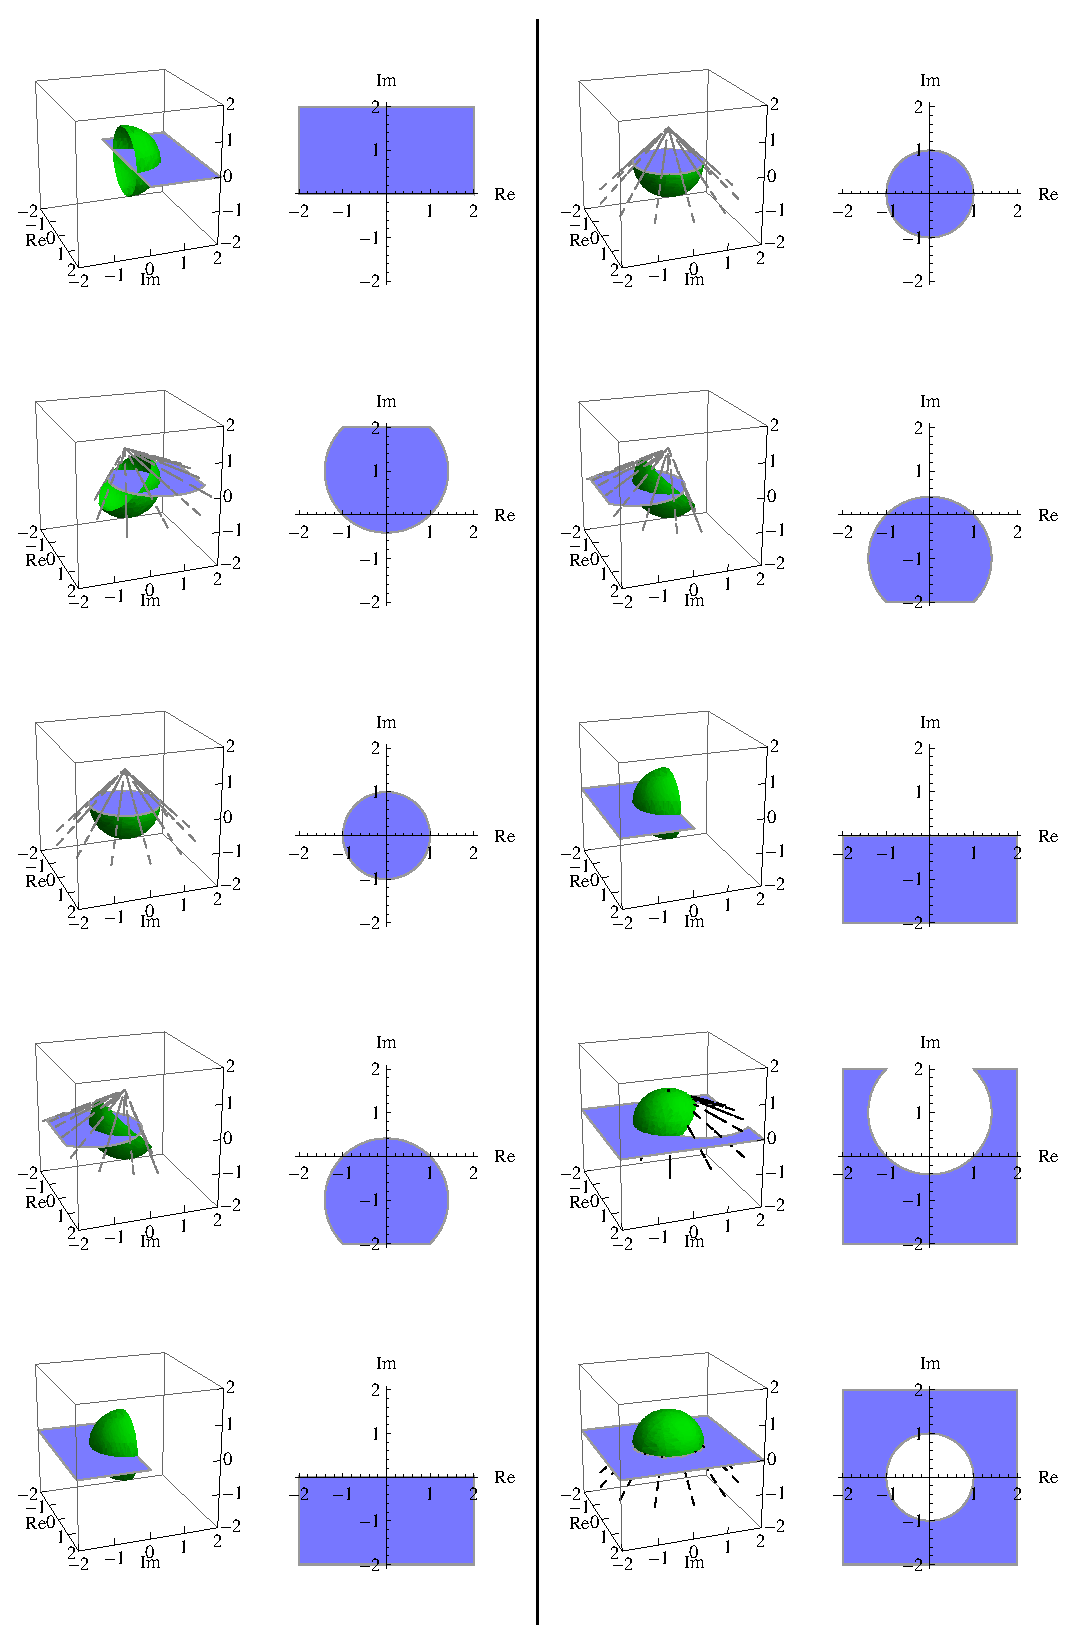
\includegraphics[width=\textwidth]{figures/stereo-proj-1}
\caption{Inversion $z \mapsto \reci{z}$ can be interpreted as rotation of the Riemann sphere by $180^{\circ}$ around the real axis. It maps the upper to the lower halfplane (left) and the unit circle to the set of numbers $\abs{z} > 1$ (right).}
\label{fig_StereoProj}
\end{figure}

\begin{remark}
\label{rem_RiemannSphere}
\index{Riemann sphere}
Stereographic projection with regard to any admissible sphere $S \subseteq \R^3$ maps $S$ bijectively to $\EC$. Of course the most natural choice for $S$ in this context is the unit sphere $\UnitSphere := \setdef{x \in \R^3}{\eucnorm{x} = 1}$ having the advantage, that stereographic projection follows the simple formula
\begin{equation}
P_{\UnitSphere}:
\begin{pmatrix} x_1 \\ x_2 \\ x_3 \end{pmatrix} 
\mapsto \frac{x_1 + \\i x_2}{1 - x_3}.
\end{equation}
Also reverse stereographic projection can be done easily using the unit sphere:
\begin{equation}
P_{\UnitSphere}^{-1}: z \mapsto 
\reci{\abs{z}^2 + 1} 
\begin{pmatrix}2 \Re{z} \\ 2 \Im{z} \\ \abs{z}^2 - 1\end{pmatrix}.
\end{equation}
By pointwise identifying $\EC$ with $S_1$ using the above two mappings, we obtain the $\emph{Riemann sphere}$ model of the extended complex plane. One of its benefits is, that certain functions $\EC \to \EC$ can be interpreted nicely as simple rotations of the Riemann sphere.
\end{remark}

\begin{example}
\label{ex_StereoProjInversion}
Consider the map $f: z \mapsto \reci{z}$. The first row of Figure~\ref{fig_StereoProj} shows the upper halfplane $U$ on the left and the unit disk $D$ on the right together with their images under reverse stereographic projection. We see that both, $U$ and $D$ correspond to a certain ``halfsphere'' of the Riemann sphere. If we rotate these halfspheres around the $x_1$ axis (leaving the points $\{\pm 1\}$ fixed) and continuously perform stereographic projection, we see that after a half turn -- in the last row of Figure~\ref{fig_StereoProj} -- we end up with $f(U)$, the lower halfplane and $f(D)$, the set of points $z$ with $\abs{z} > 1$. Thus, $z \mapsto \reci{z}$ can be interpreted as rotation of the Riemann sphere around the real axis by $180^{\circ}$.
\end{example}

Other examples for transformations corresponding to a half-turn of the Riemann sphere are $z \mapsto -z$ (rotation around the $x_3$ axis) and $T: z \mapsto -\reci{z}$ (rotation around the $x_2$ axis), a function which maps the upper halfplane to itself and which will be important in the study of the modular group -- see Section~\ref{sec_ModularGroupGenRel}.  

\begin{example}
\index{Cayley transform}
\label{ex_StereoProjCayleyMap}
In the first three rows of Figure~\ref{fig_StereoProj} on the left, the action of yet another interesting transformation can be seen, which maps the upper halfplane to the unit disk. It is given by
\begin{equation*}
f(z) = \moebius{\ii}{1}{}{\ii}{z}
\end{equation*}
and can be either considered as a quarter turn of the Riemann sphere around the real axis or as ``half of an inversion'', since indeed $f^2(z) = f(f(z)) = \reci{z}$. In contrast to its better known brother, the \emph{Cayley transform} given by
\begin{equation*}
c(z) = -\ii f(z) = \frac{z - \ii}{z + \ii},
\end{equation*}
$f$ leaves the points $\{\pm 1\}$ fixed, which often beneficial for visualization purposes.
\end{example}

We have now seen exemplarily, that rotation of the Riemann sphere induces quite a few interesting maps. If we are willing to allow not only rotations of the Riemann sphere but also translations, we indeed obtain a new characterization of M�bius transformations, as stated in the next theorem.

\begin{definition}
\index{Rigid motion}
A \emph{rigid motion} of $\R^3$ is an affine isometric transformation of $\R^3$ which is obtained purely by composition of rotations and translations.
\end{definition}

\begin{theorem}
\label{thm_MoebiusRevealed}
A function $\phi : \EC \to \EC$ is a M�bius transformation, if an only if it can be obtained by reverse stereographic projection of $\EC$ to an admissible sphere $S \subseteq \R^3$, followed by a rigid motion T of $\R^3$ which maps $S$ to another admissible sphere $TS$, followed by stereographic projection from $TS$ back to $\EC$:
\begin{equation}
\label{eqn_MoebiusRevealedForm}
\phi = P_{TS} \circ T \circ P_S^{-1}.
\end{equation}
\end{theorem}
\begin{proof}[Sketch of proof]
The fact that all maps of form ($\ref{eqn_MoebiusRevealedForm}$) are indeed M�bius transformations can be seen either by direct calculation or by the observation that $\phi$ corresponds to map $P_S \circ \phi \circ P_S^{-1} = P_S \circ P_{TS}^{-1} \circ T$ from $S$ to itself. If we identify $S$ with the Riemann sphere, we can regard $\phi$ as a holomorphic automorphism of the Riemann sphere which is therefore a M�bius transformation [REFERENCE].

It remains to show that every given transformation can indeed be realized in the form (\ref{eqn_MoebiusRevealedForm}). For this purpose, we first consider the four basic types of M�bius transformations:
\begin{description}
\item[Translation:] The map $z \mapsto z + \alpha,\ \alpha \in \C$ can be realized by choosing an arbitrary admissible sphere $S$ and setting $T = T_{\alpha}: x \mapsto x + \iota(\alpha)$, which simply translates $S$ in a direction parallel to the $x_3 = 0$ plane by $\iota(\alpha)$.
\item[Dilation:] The map $z \mapsto \rho z,\ \rho > 0$ can be obtained by choosing an arbitrary admissible sphere with north pole $n$ and setting $T = D_{\rho}: x \mapsto x + \left(0, 0, (\rho-1) n_3\right)$, which moves $S$ up- ($\rho > 1$)  or downwards ($\rho < 1$) in $x_3$ direction.
\item[Rotation:] The map $z \mapsto \epo{\ii \theta} z,\ \theta \in (-\pi, \pi]$ can be realized by choosing an arbitrary admissible sphere with center and setting 
\begin{equation*}
T = R_{\theta}: x \mapsto 
\begin{pmatrix}
\cos{\theta} & -\sin{\theta}            & 0\\
\sin{\theta} & \phantom{+}\cos{\theta}  & 0\\
0            & \phantom{+}0             & 1
\end{pmatrix}
\cdot
\begin{pmatrix}x_1 \\ x_2 \\ x_3 \end{pmatrix},
\end{equation*}
which rotates $S$ around the $x_3$ axis by an angle of $\theta$.
\item[Inversion:] We have seen in Example~\ref{ex_StereoProjInversion} that the map $z \mapsto \reci{z}$ can be realized by choosing $S$ as the unit sphere $\UnitSphere$ and setting
\begin{equation*}
T = V: x \mapsto
\begin{pmatrix}
1 & \phantom{+}0 & \phantom{+}0 \\
0 & -1           & \phantom{+}0 \\
0 & \phantom{+}0 & -1
\end{pmatrix}
\cdot
\begin{pmatrix}x_1 \\ x_2 \\ x_3 \end{pmatrix},
\end{equation*}
which is a rotation of $S$ around the $x_1$ axis by an angle of $180^{\circ}$.
\end{description}
Now, let $\phi(z) = \moebius{a}{b}{c}{d}{z}$ be an arbitrary M�bius transformation. As in the proof of Lemma~\ref{lem_MoebiusGenerators}, if $c = 0$ we may assume without restriction that $d = 1$ and therefore $\phi(z) = az + b$. Clearly this map can be realized in the form (\ref{eqn_MoebiusRevealedForm}) by starting with an arbitrary admissible sphere $S$ and take $T$ as the composition of rotation by $\arg(a)$, dilation by $\abs{a}$ (in either order), followed by translation by $b$:
\begin{equation*}
T := T_b \circ D_{\abs{a}} \circ R_{\arg(a)}.
\end{equation*}
If $c \ne 0$, we can scale the coefficients $a,b,c,d$ such that $c = 1$ and write $\phi$ in the form
\begin{equation*}
\phi(z) = a + \frac{b - ad}{z + d}.
\end{equation*}
Now we choose $S$ to be the sphere with unit radius centered at the point $\iota(-d)$ and we compose $T$ out of the following rigid motions: First, translation by $d$ transforms $S$ to the unit sphere $\UnitSphere$. Thus we can indeed apply $V$ as the second transformation in order to perform an inversion. Finally we apply rotation and dilation by the factor $b - ad$ followed by a translation by $a$:
\begin{equation*}
T := T_a \circ D_{\abs{b - ad}} \circ R_{\arg(b - ad)} \circ V \circ T_d. \qedhere
\end{equation*}
\end{proof}
